We evaluate the performance of B2BR throughout a series of experiments on controlled synthetic data.
%
The purpose of these experiments is to evaluate the ability of B2BR in terms of prediction (inside and outside the training distribution), as well as a method to recover causal factors.

The data generating process for each experiment constructs $n$ training examples according to the model $Y = (\text{snr} \cdot XE + N)F$.
%
Here, 
%\begin{itemize}
%    \item $F \in \mathbb{R}^{d_x \times d_y}$ contains entries drawn from $\mathcal{N}(0, d_x^{-1})$,
%    \item $X \in \mathbb{R}^{n \times d_x}$ contains rows drawn from $\mathcal{N}(0, \Sigma_X)$,
%    \item $N \in \mathbb{R}^{n \times d_x}$ contains rows drawn from $\mathcal{N}(0, \Sigma_N)$,
%    \item $E \in \mathbb{R}^{d_x \times d_x}$ is a binary diagonal matrix containing $n_c$ ones,
%    \item $\Sigma_X = AA^\top$, where $A \in \mathbb{R}^{d_x \times d_x}$ contains entries drawn from $\mathcal{N}(0, d_x^{-1})$,
%    \item $\Sigma_N = BB^\top$, where $B \in \mathbb{R}^{d_x \times d_x}$ contains entries drawn from $\mathcal{N}(0, d_x^{-1})$,
%\end{itemize}
    $F \in \mathbb{R}^{d_x \times d_y}$ contains entries drawn from $\mathcal{N}(0, d_x^{-1})$,
    $X \in \mathbb{R}^{n \times d_x}$ contains rows drawn from $\mathcal{N}(0, \Sigma_X)$,
    $N \in \mathbb{R}^{n \times d_x}$ contains rows drawn from $\mathcal{N}(0, \Sigma_N)$,
    $E \in \mathbb{R}^{d_x \times d_x}$ is a binary diagonal matrix containing $n_c$ ones,
    $\Sigma_X = AA^\top$ where $A \in \mathbb{R}^{d_x \times d_x}$ contains entries drawn from $\mathcal{N}(0, d_x^{-1})$,
    $\Sigma_N = BB^\top$ where $B \in \mathbb{R}^{d_x \times d_x}$ contains entries drawn from $\mathcal{N}(0, d_x^{-1})$,
and the factor $\text{snr} \in (0, \infty)$.

To simulate a wide range of experimental conditions, we vary $n \in \{500, 1000, 2000\}$, $d_x, d_y \in \{ 25, 50, 100, 150 \}$, $n_c \in \{ 5, 10 \}$, $\text{snr} \in \{ 0.2, 0.5, 0.75, 1 \}$. 
%
Each condition is simulated under $20$ different random seeds. 

We compare the performance of B2BR against five competing methods:
%
Ridge regression \citep{hoerl1959optimum}, multitask Lasso \citep{argyriou2008convex}, Partial Least Squares or PLS \citep{wold_pls, tenenhaus_pls}, Canonical Correlation Analysis or CCA \citep{cca_hotelling}, and Reduced Rank Regression or RRR \citep{Izenman_rrr}.
%
Each of these methods estimates a matrix of coefficients $\hat{W} \in \mathbb{R}^{d_x \times d_y}$, from which we estimate the diagonal mask $\hat{E}$ using the feature importances $\hat{E}_{i,i} = \| W_{i, :} \|$.
%
For B2BR, we obtain $\hat{E}$ as described in Algorithm~\ref{algorithm:b2br}.
%
We employ $5$-fold cross-validation to select the optimal hyper-parameters of each method. 

We evaluate seven metrics: 
%
test error in-distribution, test error out-distribution, test error-in distribution after weighting with $\hat{E}$, test error out-distribution after weighting with $\hat{E}$, Sonquist-Morgan false positives on $\hat{E}$, Sonquist-Morgan false negatives on $\hat{E}$, and the area under the ROC curve (AUC) between $\hat{E}$ and $E$.
%
The ``in-distribution'' metrics measure the test error of each predictor before and after weighting their features by the estimated mask $\hat{E}$.
%
The ``out-distribution'' metrics are similar, measuring the test error at samples drawn using two different random covariance matrices for both $X$ and $N$.
%
The false positives, false negatives, and AUC statistics measure the quality of identification of causal factors between $\hat{E}$ and the true, binary $E$. 

\begin{figure}[htpb]
    \centering
    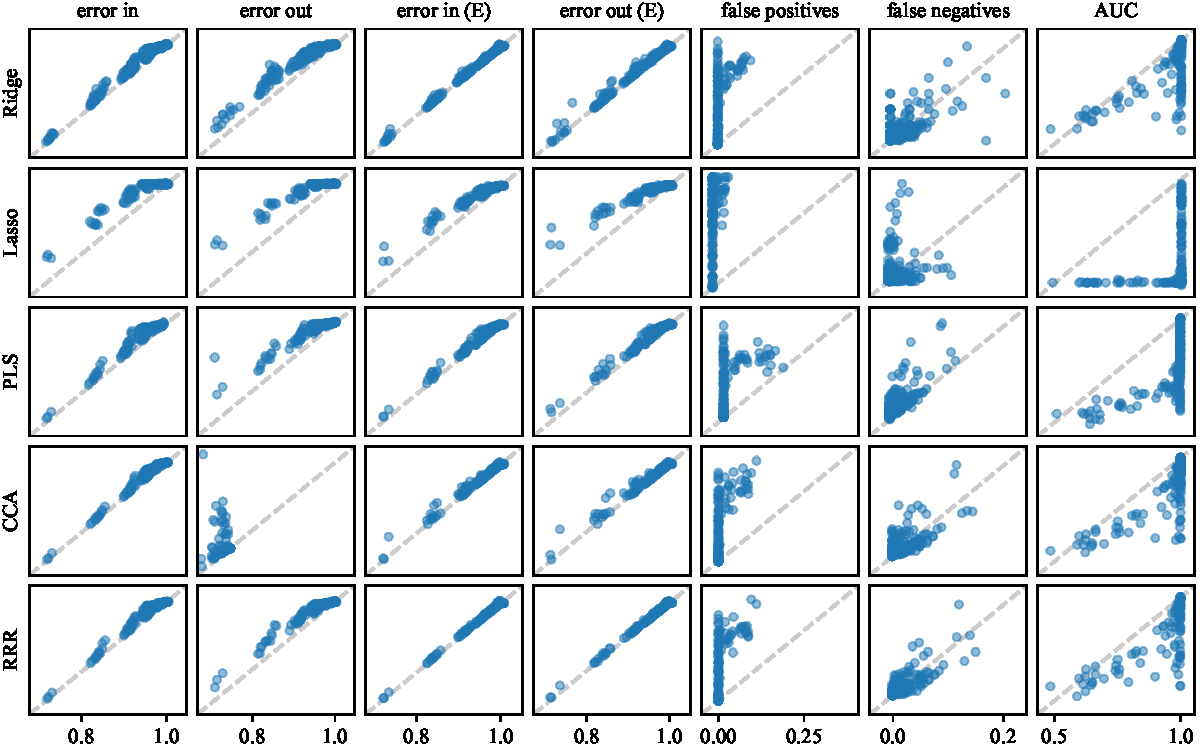
\includegraphics[width=\textwidth]{synthetic.pdf}
    \caption{Results of synthetic experiments. Each dot depicts the average value of a metric for JRR ($x$-axis) against a competitor ($y$-axis) for each experiment configuration, $20$ random seeds.}
    \label{table:synthetic}
\end{figure}

Table~\ref{table:synthetic} summarizes the results for all experimental conditions, metrics, and methods.
%
B2BR is the method obtaining best test error out-distribution, lowest false positive and false negative discovery about $E$, and overall the best AUC when it comes to detecting causal influences.

